\section{Our conclusions}
\subsection{Identity federations with SAML2 and DANE}
We started out with the task to identify where we could improve security within idenitity federations.
We specifically looked into the data integrity part of SAML2, how X.509 certificates are used and how it would be possible to improve security with the help of DNS-Based Authentication of Named Entities.

Our conclussion is that as soon as the initial configuration for each entity in an identity federation is done and all 
entities are up and running, data integrity is as secure as the public/private key cryptography scheme.
However, the difficulty is still in the initial setup, how to decide who to trust when you don't trust anyone online. 
As well as building trust when performing an emergency key rollover, when the key one day unexpectedly becomes invalid. 
Procedures for this is as of today not specified in any detail, it's up to each federation to decide on their own.
Common practice is as said in earlier chapters to share key or certificate information in some out-of-band way e.g. meeting in person or call each other.
We belive that it is this initial sharing of information that would benefit the most if it could be done solely over the internet and it's possible if we put trust in the DNSSEC infrastructure.

DANE is one way to go and is a valid solution for identity federations.
However, exactly how to store SAML2 certificates and how to retrieve the correct certificate for each validation of metadata is still an open question since we haven't been able to reach that far.
We have listed some solutions such as using CERT resource records and perhaps locating the correct certificate with "Dynamic Delegation Discovery System (DDDS)" procedures.

Furthermore, our belief is that within future SAML specifications and/or when establishing new federations, more strict rules concerning metadata must be agreed upon to secure the data integrity of the metadata.
Future agreements should include requirements that TLS with TLSA validation is used when sharing metadata.
Another requirement should be to publish the certificates within the DNS/DNSSEC infrastructure.
This is to make sure that both the channel that the communication is taking part over is secure as well as the data stored on the webserver accessed is the proper one e.g. if downloading a certificate over a HTTPS connection.

\subsection{How DANE can be implemented in Shibboleth}
\begin{figure}[ht]
\begin{center}
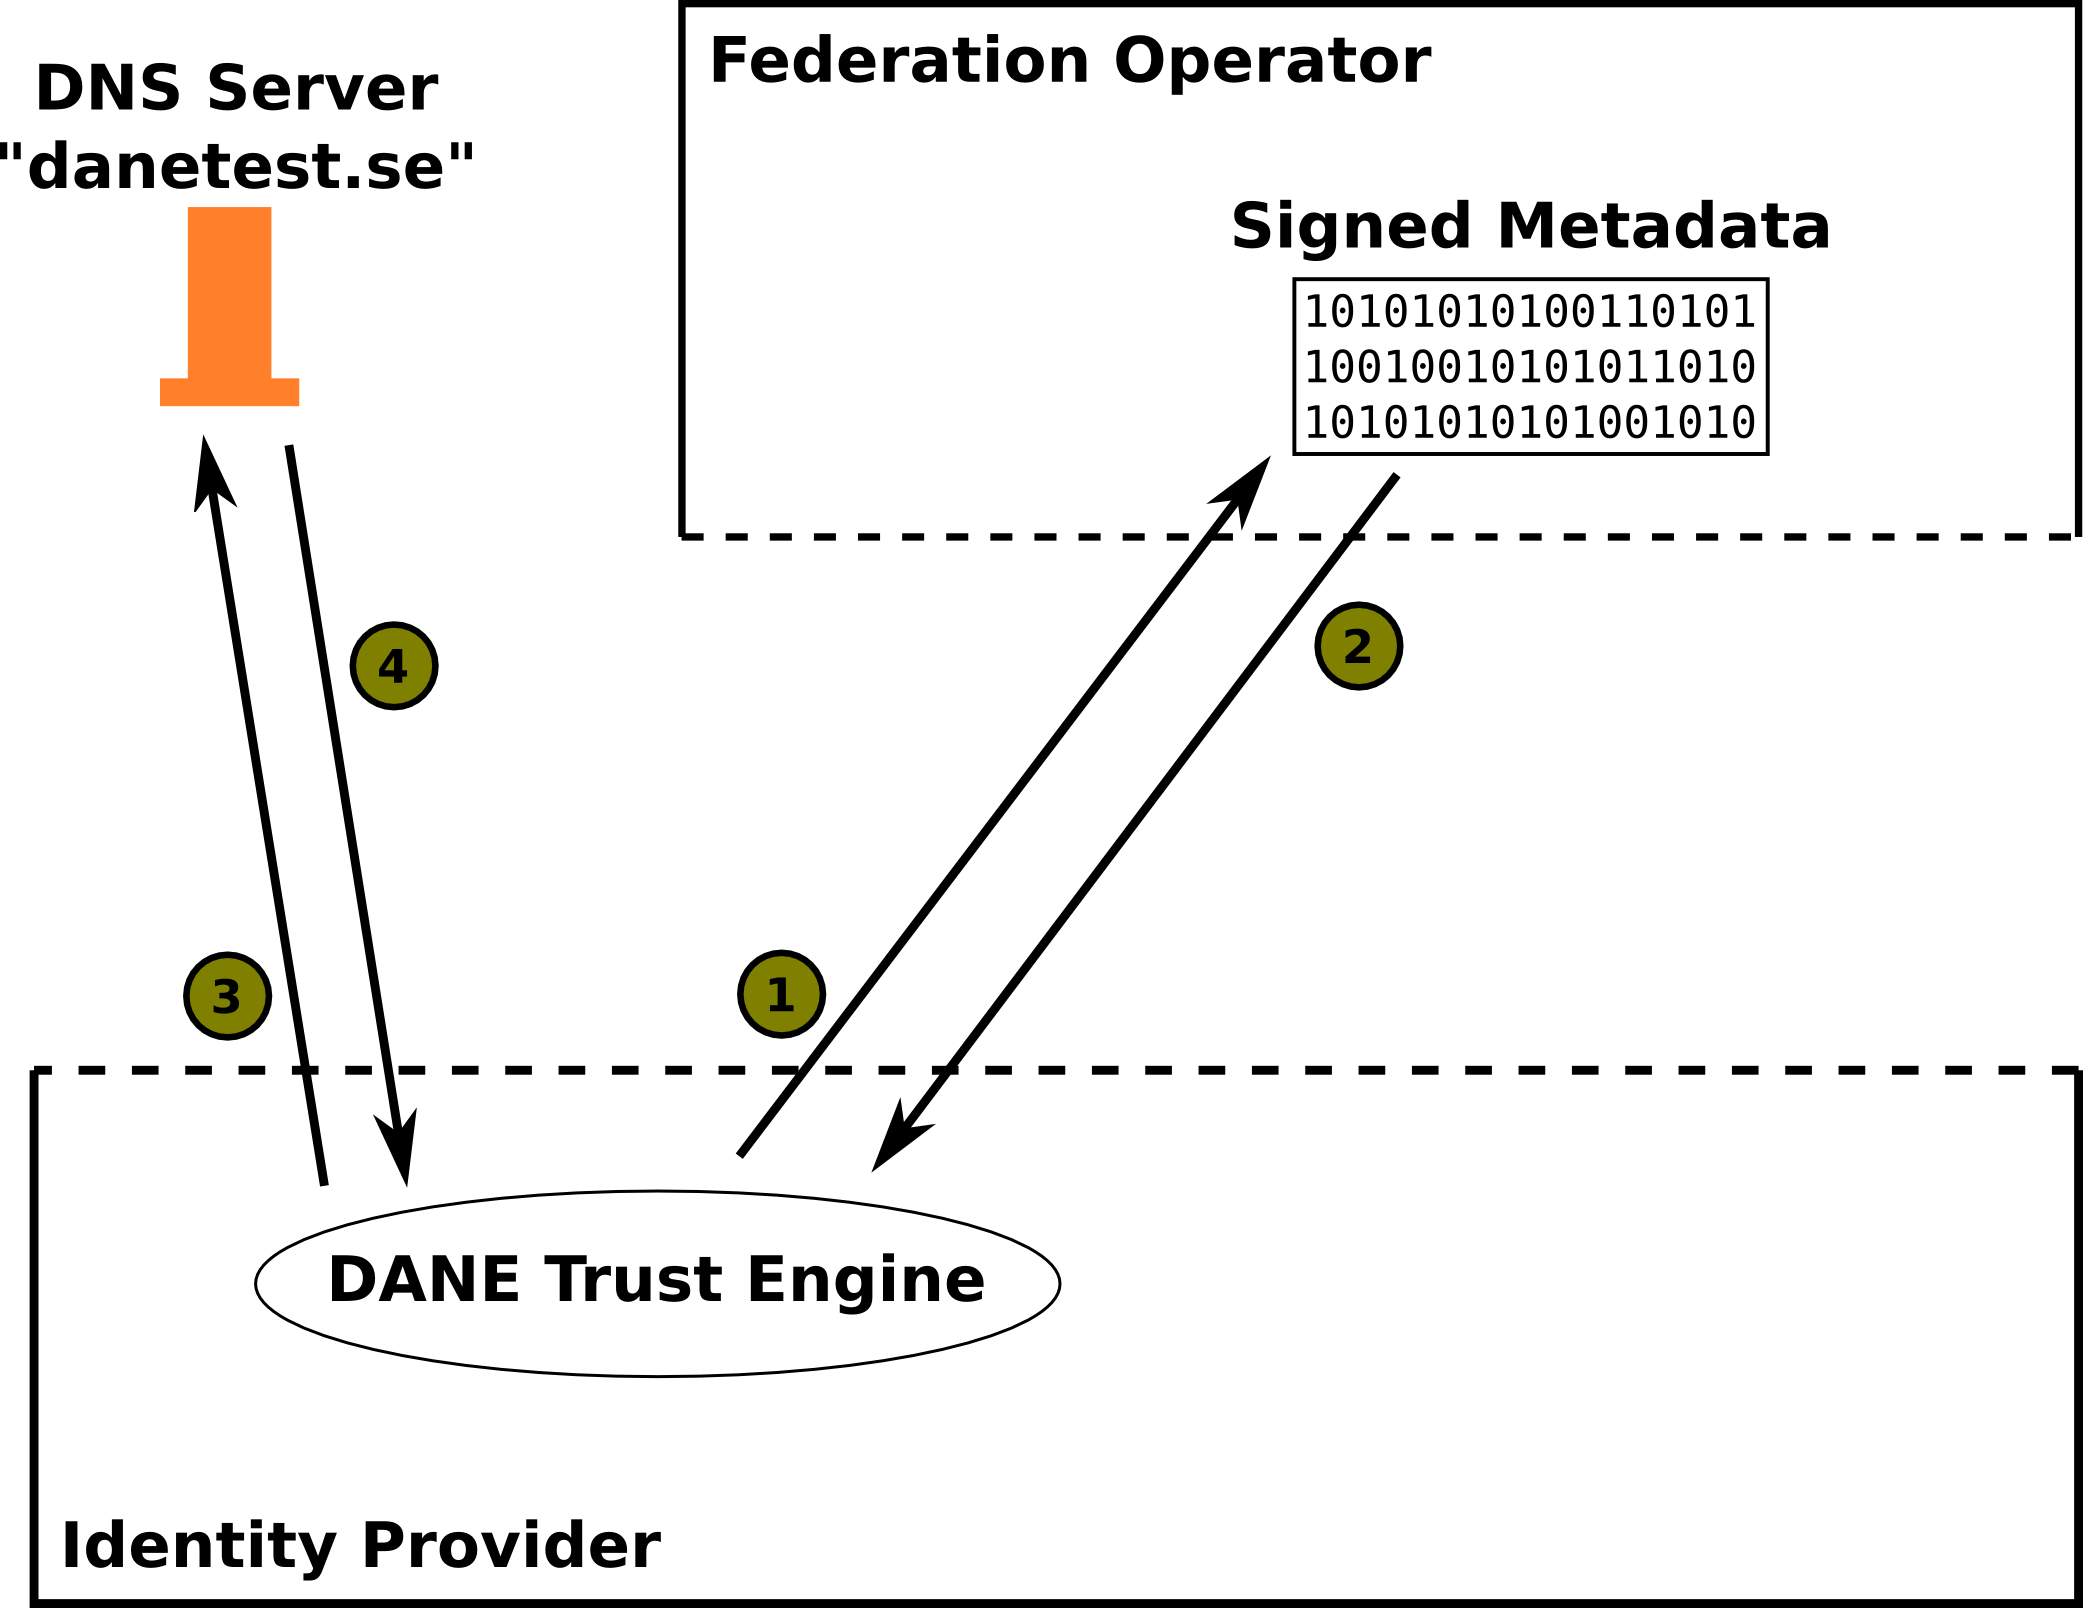
\includegraphics[scale=1]{Figures/dane-impl.png}
\end{center}
\caption{Four steps corresponding to the requests/responses vital to the DANE Trust Engine.
\label{ch5:dane-impl}}
\end{figure}


To start of at the right level we need to restate that DANE as of today, has no standard nor draft available outside the topic of TLS or S/MIME communication.
What we set out to implement is more of a proof-of-concept that when/if there is a standard available for SAML certificates, or perhaps certificates in general, our implementation might be a solution to build upon.
It's also important to remember that we have only looked at the identity provider software out of all computer programs available under the Shibboleth name.
When/If DANE would be implemented into Shibboleth, development has to be made to all parts that publish and consume metadata.

We started out focusing on developing a metadatafilter extension for Shibboleth.
After some digging it became clear that it would be a trust engine extension that was better suited for our purpose.

% TODO: Is this the right way to go?
Our DANE trust engine is intended to be configured from the standard xml-configuration files. 
The trust engine recieves the metadata as argument (Step 1 and 2 in figure \ref{ch5:dane-impl}) and then requests a CERT RR from the domain name system with the DNSSEC flags set (Step 3 in the same figure). 
If the reponse comes back without DNSSEC flags set the information is not to be trusted otherwise it will compare the certificate retrieved with the one supplied as argument.
Depending on the outcome of that comparison the trust engine will either confirm or dismiss trust for the metadata.

Due to time constraints and limited previous knowledge in Java/Spring Framework we were unable to finish the implementation in time.
Installation and configuration guides are available in appendix \ref{appA} as well as references to our code available online.

% Why do we give credentials as input from the configuration file? Kommer inte det finnas i Metadatan som vi jämför med CERT RR.
%It's worth mentioning that (1) signing of cert rr possible? (2) perhaps better implementations directly witin OpenSSL or OpenSAML.

%DANE
%Säkra både TLS och certifikat eftersom webbserver kan hackas men inte så troligt att även zonen blir hackad eftersom det är vanligt att placera en master server bakom många slav-servrar som är blåttade mot omvärlden.


%Connect back to the topic under "Chapter 1: Purpose". Do we reach our purpose?
% TODO: Make comments about that if we can secure the transmission of Metadata between all entities (FOs, IdPs, AAs, SPs and Discos) we can deem that the data integrity of all messages transmitted between them(the entities) is not lost or tampered with. As long as all entities do a proper check for each SAML2 message.

\section{How to continue with further research}
\subsection{Secure communication with a federation operator}
The communication between the federation operator and the other entities such as identity providers and service providers has no standardized way in how it should work.
How does the federation operator know that it really is the right identity provider it's talking with, without any prior communication?
Should the federation operator be the one that initiate connection to the other entities or vice versa?
Last, but not least, how should this be solved technically to minimize the manual labour and automate as much as possible?

\subsection{Publishing SAML2 certificate as CERT RR, is it viable?}
In section \ref{subsec:saml2-certs-in-cert-rr} it's mentioned that SAML2 certificates could be stored in CERT RRs.
Further research need to be done to establish exactly how this could be accomplished.
With CERT RR it's possible to store the certificate in it's full format, only a hash of it or just a url to the location where it's stored\cite[ch. 2.1]{rfc:4398}.
What would be suitable for SAML2 certificates and is this really a viable solution for the identity federation scheme?

\subsection{How to locate the correct certificate in DNS}
In section \ref{subsec:matching-dilemma} "Dynamic Delegation Discovery System (DDDS)"\cite{rfc:3401,rfc:3402,rfc:3403,rfc:3404} and the NAPTR resource record\cite{rfc:3403} is mentioned as a possible solution to the "matching problem".
How does an entity that has recieved a signed metadata file locate the correct certificate within the Domain Name System?

%\section{Temporary section }
%DISCUSSION Your conclusions, where you link your findings to your theories and purpose,
%will discuss whether you achieved your purpose and what opportunities exist for further
%development. An analysis and interpretation of your results may often correspond to the
%frame of reference and the theoretical models you have used. Using models, checklists etc,
%you broke down your task into manageable questions. Now you reverse your approach and
%use them to build general conclusions and recommendations that correspond to your
%purpose and your client's decision situation.

